\begin{figure}[H]
    \centering
    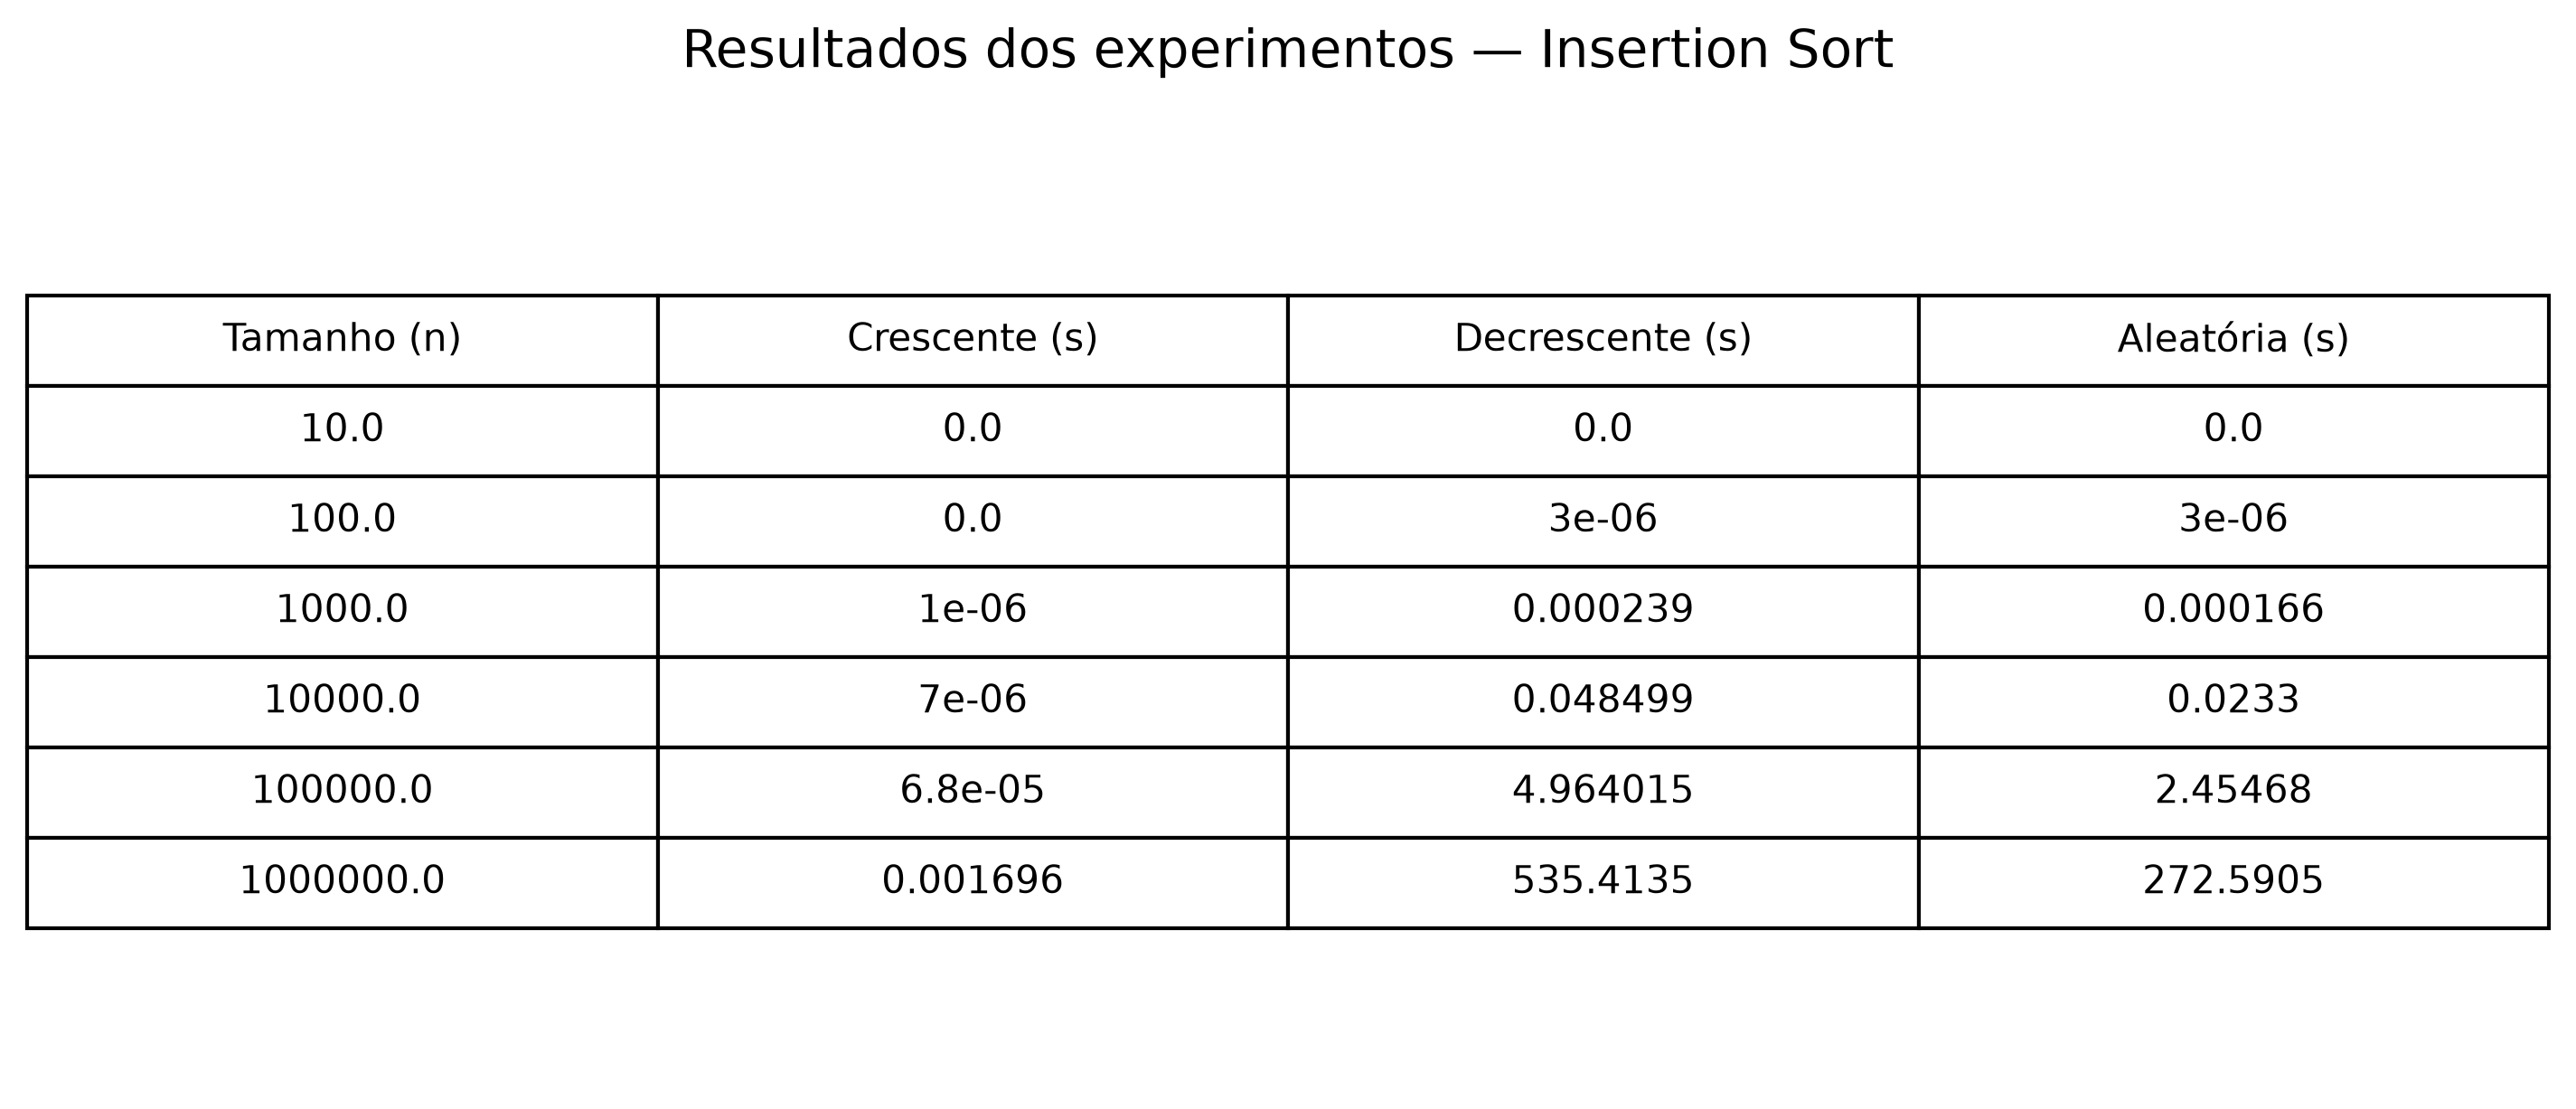
\includegraphics[width=16cm]{Imagens/Insertion_Sort/tabela.png}
    \caption{Tabela de tempo de execução do algoritmo Insertion Sort}
    \label{fig:tabela-insertion}
\end{figure}

\begin{figure}[H]
    \centering
    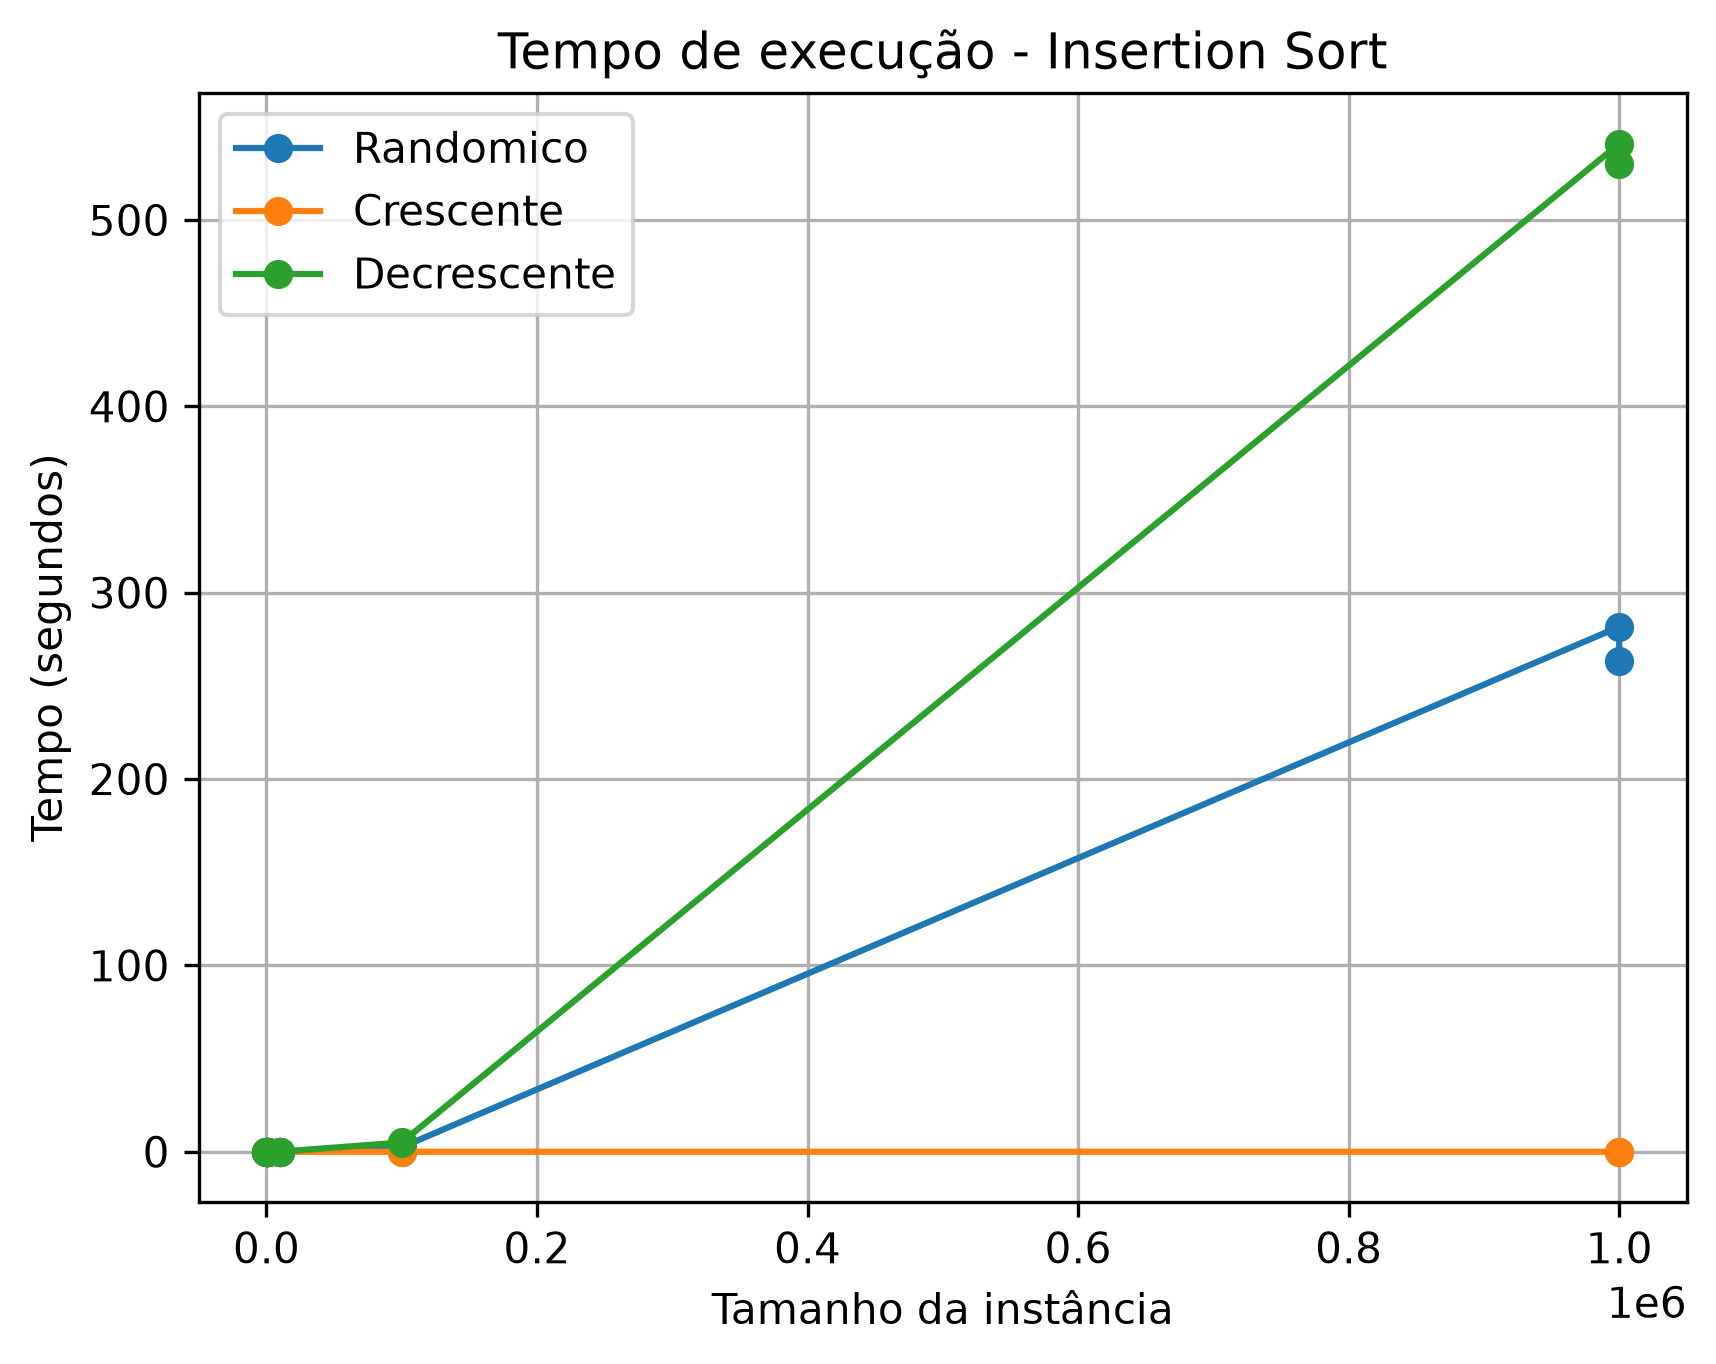
\includegraphics[width=10cm]{Imagens/Insertion_Sort/grafico.png}
    \caption{Gráfico de tempo de execução do algoritmo Insertion Sort}
    \label{fig:grafico-insertion}
\end{figure}

Os resultados obtidos nos experimentos estão apresentados na tabela e no
gráfico. Observa-se que o algoritmo Insertion Sort apresenta melhor
desempenho para instâncias ordenadas de forma crescente, uma vez que,
nesse caso, praticamente não são necessárias movimentações dos elementos.

Em contrapartida, as instâncias ordenadas de forma decrescente apresentam
os maiores tempos de execução. Isso ocorre porque cada novo elemento
precisa ser comparado e deslocado por uma grande quantidade de posições,
caracterizando o pior caso do algoritmo, cuja complexidade é
$\Theta(n^2)$.

As instâncias aleatórias apresentam desempenho intermediário, pois a
quantidade de deslocamentos depende da disposição inicial dos elementos.

A partir dos dados, também é possível perceber que o aumento do tamanho
da entrada provoca um crescimento significativo no tempo de execução,
principalmente nos casos aleatório e decrescente. Para a instância de
tamanho $n = 1.000.000$, o tempo registrado foi aproximadamente
$272{,}59$ segundos para a entrada aleatória e $535{,}41$ segundos para a
entrada decrescente. Já para a entrada crescente, o tempo foi de
aproximadamente $0{,}001696$ segundos.

Esses resultados confirmam o comportamento teórico esperado para o
algoritmo Insertion Sort.